
\documentclass[letterpaper, 10 pt, conference]{ieeeconf}  % Comment this line out if you need a4paper
\IEEEoverridecommandlockouts                              % This command is only needed if 
                                                          % you want to use the \thanks command
\overrideIEEEmargins                                      % Needed to meet printer requirements.


% Bibliography
\usepackage{biblatex}
\addbibresource{references.bib}

% Math
\usepackage{physics}
\usepackage{siunitx}
\sisetup{output-exponent-marker=\ensuremath{\mathrm{e}}}
\usepackage{amsmath}
\usepackage{amsfonts}
\usepackage{amssymb}

% Optimization and Algorithms
\usepackage{optidef}
\usepackage{algorithmicx}
\usepackage{algorithm,algpseudocode}

% Formatting
\usepackage{xcolor}
\usepackage{bm}  % for bold symbols 
\usepackage{booktabs}  % better tables
\usepackage{pifont}  % for x mark
\usepackage{graphicx}
\usepackage{hyperref}

% Plotting
\usepackage{pgfplots}
\pgfplotsset{compat=1.15,
	legend style={font=\footnotesize},
}
\usepackage{tikzscale}

% Custom commands
\newcommand{\half}{\frac{1}{2}}
\newcommand{\R}{\mathbb{R}}
\newcommand{\Q}{\mathbb{S}^3}
\newcommand{\skewmat}[1]{[#1]^\times}

\newcommand{\rmap}{\varphi}
\newcommand{\invrmap}{\varphi^{-1}}

\newcommand{\dR}{\delta \mathcal{R}}
\newcommand{\rot}{ \mathcal{R} }
\newcommand{\dq}{\delta q}
\newcommand{\q}{\textbf{q}}
\newcommand{\eq}{_\text{eq}}
\newcommand{\traj}[2][N]{#2_{0:{#1}}}
\newcommand{\pass}{{\color{green} \checkmark}}
\newcommand{\fail}{{\color{red} \ding{55}}}

\newcommand{\todo}[1]{\textcolor{red}{TODO: #1}}


\title{\LARGE \bf
Planning with Attitude
}

\author{Brian Jackson$^1$ and Zachary Manchester$^1$%
    \thanks{
        $^1$Robotics Institute, 
        Carnegie Mellon University, 
        5000 Forbes Ave, Pittsburgh, PA, USA
    }
}

\begin{document}
\maketitle

\section{INTRODUCTION} 

    Many useful robotic systems---including quadrotors, airplanes, satellites, autonomous
    underwater vehicles, and quadrupeds---can perform arbitrarily large three-dimensional
    translations and rotations as part of their normal operation. While simply
    representing the attitude of these sytems is nontrivial, generating and tracking
    motion plans for floating-base systems is an even more challenging problem.

    Many approaches \todo{add some citations here} have been taken to address the problem of motion planning and control
    on the $SE(3)$ group; most of these rely heavily on ideas and notation
    from differential geometry. Despite some impressive results, many of these ideas
    have not been widely adopted by the robotics community, and many practitioners continue to ignore the group structure of rotations. One issue preventing wider adoption is that accounting for this structure requires low-level changes to the underlying
    optimization algorithms, which is difficult or impossible when relying on existing
    off-the-shelf solvers.
    
    \todo{I'm worried that SE(3) and SO(3) results are getting confused/conflated here. I would explicitly talk about both, emphasize that we're handling SO(3) with the quaternion stuff, and that $SE(3) = SO(3) \times \mathbb{R}^3$ is a straightforward extension.}

    To address this lack of solver support, we formulate a straightforward, generic method for adapting
    existing Newton and gradient-based algorithms to correctly account for the group structure of
    rotations. Based entirely on basic mathematical tools from linear algebra and
    calculus, our method is computationally efficient and should be both accessible and
    familiar to most roboticists. We apply this method to the ALTRO solver
    \cite{howell2019altro} and demonstrate its performance on several constrained trajectory
    optimization problems.

\section{Notation and Convensions}

    We begin by defining some useful conventions and notation. 
    Attitude is defined as the rotation from the robot's body frame to a global inertial 
        frame. 
    We also define gradients to be row vectors, that is, for 
        $f(x) : \R^n \to \R$, $\pdv{f}{x} \in \R^{1\times n}$.

    We represent---following the Hamilton convention---a quaternion $\q \in \mathbb{H}$ as 
    a standard vector $q \in \R^4 := [q_s \;\; q_v^T]^T$ where $q_s \in \R$ and 
    $q_v \in \R^3$ are the scalar and vector part of the quaternion, respectively. We denote
    the composition of two quaternions as $q_3 = q_2 \otimes q_1$.
        
        % Quaternion multiplication is defined as
        % \begin{equation} \label{eq:quat_mult}
        %     \q_2 \otimes \q_1 = L(q_2) q_1 = R(q_1) q_2
        % \end{equation}
        % where $L(q)$ and $R(q)$ are orthonormal matrices defined as
        % \begin{align}
        %     L(q) &:= \begin{bmatrix} 
        %         q_s \;\; & -q_v^T \\ 
        %         q_v \;\; & q_s I + \skewmat{q_v} 
        %     \end{bmatrix} 
        %     \label{eq:Lmult} \\
        %     %= \begin{bmatrix} q & G(q) \end{bmatrix} \label{eq:Lmult} \\
        %     R(q) &:=\begin{bmatrix} 
        %         q_s \;\; & -q_v^T \\ 
        %         q_v \;\; & q_s I - \skewmat{q_v} 
        %     \end{bmatrix} \label{eq:Rmult},
        % \end{align}
        % and $\skewmat{x}$ is the skew-symmetric matrix operator
        % \begin{equation}
        %     \skewmat{x} := \begin{bmatrix} 
        %         0 & -x_3 & x_2 \\ 
        %         x_3 & 0 & -x_1\\ 
        %         -x_2 & x_1 & 0 
        %     \end{bmatrix}.
        % \end{equation}
        
        % The inverse of a unit quaternion $q^{-1}$, giving the opposite rotation, is equal 
        % to its conjugate $q^*$, which is simply the same quaternion with a negated vector 
        % part:
        % \begin{equation} \label{eq:T}
        %     \q^* = T q := \begin{bmatrix} 
        %         1 & \\ 
        %         & -I_3 
        %     \end{bmatrix} q
        % \end{equation}
        % The following identities, which are easily derived from 
        % \eqref{eq:Lmult}--\eqref{eq:T}, are extremely useful:
        % \begin{align}
        %     &L(Tq) = L(q)^T = L(q)^{-1} \\
        %     &R(Tq) = R(q)^T = R(q)^{-1} .
        % \end{align}
        
        % We will sometimes find it helpful to create a quaternion with zero scalar part from 
        % a vector $r \in \R^3$. We denote this operation as,
        % \begin{equation}
        %     \hat{r} = H r \equiv \begin{bmatrix} 0 \\ I_3 \end{bmatrix} r.
        % \end{equation}
        % Unit quaternions rotate a vector through the operation 
        % $\hat{r}' = \q \otimes \hat{r} \otimes \q^*$. 
        % This can be equivalently expressed using matrix multiplication as
        % \begin{align} 
        %     r' &= H^T L(q) R(q)^T H r = A(q)r , \label{eq:quaternion_rotation}
        % \end{align}
        % where $A(q)$ is the rotation matrix in terms of the elements of the quaternion 
        % \cite{markley2014fundamentals}. 

\section{Quaternion Differential Calculus} \label{sec:Quaternion_Calculus}
    Most modern methods for planning and control require derivatives with respect to the
    state vector. We present a simple but powerful method for taking derivatives of 
    quaternion-valued state vectors. The extension of this method to more general state vectors that contain Cartesian products of $SO(3)$, $SE(3)$, and $\mathbb{R}^n$ is straightforward.

    The key idea of this section is that differential quaternions live in three-dimensional
    space instead of the four-dimensional space of quaternions. This can be seen graphically
    (see Figure \ref{fig:tangent_plane}) or deduced intuitively, since rotations are
    inherently three-dimensional and differential rotations should live in the same space as 
    angular velocity, i.e. $\R^3$.

    \begin{figure}
        \centering
        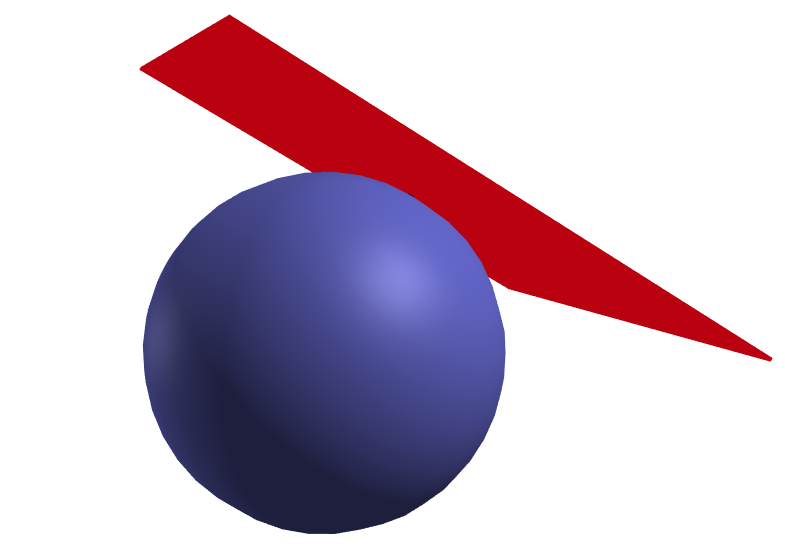
\includegraphics[height=5cm]{figures/tangent_plane.tikz}
        \caption{
            When linearizing about a point $q$ on an sphere $\mathbb{S}^{n-1}$ in 
            n-dimensional space, the tangent space $T$ is a hyper-plane $\R^{n-1}$, 
            illustrated here with $n=3$. Therefore, when linearizing about a unit 
            quaternion $q \in \Q$, the space of differential rotations lives in $\R^3$.
        }
        \label{fig:tangent_plane}
    \end{figure}
    In practice, we have found Rodrigues Parameters to be a very effective representation
    for three-dimensional differential rotations since they are computionally efficient
    and do not inherit the sign ambiguity of quaternions.
    
    The mapping between a vector of Rodrigues parameters $\phi \in \R^3$ and a unit
    quaternion $q$ is known as the Cayley map:
    \begin{equation} \label{eq:cayley}
        q = \varphi(\phi) = \frac{1}{\sqrt{1 + \norm{\phi}^2}} \begin{bmatrix} 1 \\ \phi \end{bmatrix}.
    \end{equation}
    We will also make use of the inverse Cayley map:
    \begin{equation} \label{eq:invcayley}
        \phi = \varphi^{-1}(q) = \frac{q_v}{q_s}.
    \end{equation}

    \subsection{Jacobian of Vector-Valued Functions}
        When taking derivatives with respect to quaternions, we must take into account
        both the composition rule and the nonlinear mapping between the space of unit
        quaternions and our chosen three-parameter error representation.

        Let $\phi \in \R^3$ be a differential rotation applied to a function with
        unit quaternion inputs $y = h(q): \Q \to \R^p$, such that
        \begin{equation} \label{eq:vector_function}
            y + \delta y = h(q \otimes \varphi(\phi)) \approx h(q) +  \nabla h(q) \phi.
        \end{equation}
        We can calculate the Jacobian $\nabla h(q) \in \R^{p \times 3}$ by
        differentiating \eqref{eq:vector_function} with respect to $\phi$, evaluated at
        $\phi = 0$:
        \begin{equation} \label{eq:quat_gradient}
            \nabla h(q) = \pdv{h}{q} \begin{bmatrix} 
                            -q_v^T \\ 
                            sI_3 + \skewmat{q_v}
                        \end{bmatrix}
                        := \pdv{h}{q} G(q) 
        \end{equation}
        where $G(q) \in \R^{4 \times 3}$ is referred to as the \textit{attitude Jacobian}, which
        essentially becomes a ``conversion factor'' allowing us to apply results from
        standard vector calculus to the space of unit quaternions. This form is
        particularly useful in practice since $\pdv*{h}{q} \in \R^{p \times 4}$ can be
        obtained using finite difference or automatic differentiation.
        As an aside, although we have used Rodrigues parameters, $G(q)$ is actually the
        same (up to a constant scaling factor) for any choice of three-parameter attitude
        representation.

    \subsection{Other derivatives}
        Using similar techniques, we find useful expressions for the Hessian of a
        scalar-valued function (i.e. $p = 1$):
	    \begin{equation} \label{eq:quat_hessian}
            \nabla^2 h(q) = G(q)^T \pdv[2]{h}{q} G(q) + I_3 \pdv{h}{q}q,
        \end{equation}
        and the Jacobian of a quaternion-valued function $q' = f(q) : \Q \to \Q$:
        \begin{equation} \label{eq:quat_jacobian}
            \nabla f(q) = G(q')^T \pdv{f}{q} G(q).
        \end{equation}


\section{Fast Constrained Trajectory Optimization on $SE(3)$}
    \subsection{Algorithmic Modifications}
    Here we briefly outline the changes to the ALTRO solver \cite{howell2019altro} to 
    efficiently solve trajectory optimization problems for systems with 3D rotations in the
    state vector. 
%     The AL-iLQR algorithm at the heart of ALTRO requires linearization of the
%     dynamics ($A \in \R^{n \times n}, B \in \R^{n \times m}$), the constraints ($\c_x \in 
%     \R^{p \times n}, c_u \in \R^{p \times m}$), and a quadratic expansion of the cost
%     function ($Q \in \R^{n \times n}, R \in \R^{m \times m}, q \in \R^n, r \in \R^m$). These
%     can be computed as follows:
    The linearization of the nonlinear discrete dynamics function $x_{k+1} = f(x_k,u_k)$ is 
    ``corrected'' using \ref{eq:quat_jacobian}:
    \begin{equation}
        A = G(f(x,u))^T \pdv{f}{x} G(x); \quad B = G(f(x,u))^T \pdv{f}{u}.
    \end{equation}
    We can similarly compute the linearization of a nonlinear constraint function $c(x,u)$
    using \ref{eq:quat_gradient}:
    \begin{equation}
        c_x = \pdv{c}{x} G(x); \quad c_u = \pdv{c}{x}.
    \end{equation}
    Lastly, we adjust the computation of the quadratic expansion of the augmented
    Lagrangian \todo{I would leave out the AL stuff and just talk about a generic cost function here to make it more general} cost function $J(x,u) + \lambda^T c(x,u) + \half c(x,u)^T I_\mu c(x,u)$
    using \ref{eq:quat_gradient} and \ref{eq:quat_hessian}:
    \begin{subequations}
        \begin{align}
            Q &= & G(x)^T & \pdv[2]{J}{x} G(x) + c_x^T I_\mu c_x + I_3 \pdv{J}{x} x \\
            R &= &        & \pdv[2]{J}{u}      + c_u^T I_\mu c_u \\
            H &= &        & \pdv{J}{u}{x} G(x) + c_u^T I_\mu c_x \\
            q &= & G(x)^T & \pdv{J}{x} + c_x^T (I_\mu c(x,u) + \lambda) \\
            r &= &        & \pdv{J}{u} + c_u^T (I_\mu c(x,u) + \lambda).
        \end{align}
    \end{subequations}
    Here we define the \textit{state attitude Jacobian} $G(x)$ to be a block-diagonal
    matrix where the block is an identity matrix for any vector-valued state and $G(q)$ for
    any quaternion in the state vector. We refer the reader to the original ALTRO paper 
    \cite{howell2019altro} for futher details on the algorithm.

    These adjustments effectively modify the optimization so that it is performed on the
    quaternion error state (or Rodrigues Parameters) instead of the space of unit
    quaternions. In practice, this is analagous to the Multiplicative Extended Kalman
    Filter \cite{markley2014fundamentals} in the state estimation community.

    The algorithm only needs one small modification to the ``forward pass,'' where the
    trajectory is modified by simulating the system forward using the optimal feedback
    policy, $\delta u = K \delta x + d$, computed during the ``backward'' pass. Instead of 
    computing $\delta x$ using simple subtraction, we now compute the error state using the
    inverse Cayley map \eqref{eq:invcayley} for the quaternion states. The rest of the
    forward pass is unmodified. \todo{I think you can safely omit some of these details and just refer to the ALTRO paper.}

    \subsection{Examples}
        To demonstrate the effectiveness of the proposed approach, we ran the modified
        version of ALTRO on several problems involving arbitrary 3D orientations. One 
        required a quadrotor to do an aggresive ``zig-zag'' pattern, another to do a flip,
        and the last tasked a model airplane model to do a barrell roll. The timing results
        are shown in Figure \ref{fig:timing_chart}.
        \begin{figure}
            \centering
            \includegraphics[height=4cm, width=8cm]{figures/timing_chart.tikz}
            \caption{Timing results for the airplane barrell roll, quadrotor flip, and
            quadrotor zig-zag examples using iLQR with roll-pitch-yaw Euler angles (RPY),
            quaternions, and the current method. The timing result for the Quadrotor flip
            with Euler angles is omitted since it failed to converge.
            }
            \label{fig:timing_chart}
        \end{figure}
        
        \todo{It would be great to compare to both the minimal iLQR stuff and SNOPT or IPOPT with quaternion norm constraints + slack variables (referred to as the ``embedding approach'').}

\section{Conclusion} 

    We have proposed a general, accessible, and computationally efficient approach to
    doing planning and control for systems with one or more unit quaternions in their
    state vectors. The approach allows for straightforward adaptation of many
    gradient-based methods for optimal control and motion planning, which we demonstrated
    on the ALTRO solver. We have demonstrated that correctly leveraging the group
    structure of rotations results in lower solve times and improved robustness of the
    optimization algorithm.

        
% \section{Multiplicative LQR} \label{sec:MLQR}
%     Leveraging the methods from the previous section, we derive multiplicative LQR
%     (MLQR), a variant of LQR that correctly accounts for the group structure of
%     rotations. For concreteness, we consider a system with rigid body dynamics, as
%     presented in Sec. \ref{sec:rigidbody_dynamics}, and design a controller to stabilize
%     the system about a dynamically feasible discretized reference trajectory
%     $\bar{x}_{0:N}, \bar{u}_{0:N}$ with $N$ time steps.
%     We begin by linearizing the dynamics about the reference trajectory using \eqref{eq:quat_jacobian}. Our linearized error dynamics become
%     \begin{equation} \label{eq:linearized_dynamics}
%         \delta x_{k+1} = A_k \delta x_k + B_k \delta u_k 
%     \end{equation}
%     where \begin{equation}
%         \begin{aligned}
%             A_k = E(\bar{x}_{k+1})^T \pdv{f}{x}|_{\bar{x}_k,\bar{u}_k} E(\bar{x}_k), \\
%             B_k = E(\bar{x}_{k+1})^T \pdv{f}{u}|_{\bar{x}_k,\bar{u}_k},
%         \end{aligned}
%     \end{equation}
%     and $\delta x_k \in \R^{12}$ and $E(x_k) \in \R^{12 \times 13}$ are the state error and state error Jacobian:
%     \begin{equation} \label{eq:state_error}
%         \setlength\arraycolsep{1pt}
%         \delta x_k = \begin{bmatrix} 
%             r_k - \bar{r}_k \\ \varphi^{-1}(\bar{\q}_k^{-1} \otimes \q_k) \\ v_k - \bar{v}_k \\ \omega_k - \bar{\omega}_k 
%         \end{bmatrix}\!, \;
%         E(x) = \begin{bmatrix}
%             I_3 & & & \\
%             & G(q) & & \\
%             & & I_3 & \\
%             & & & I_3 \\
%         \end{bmatrix}\!.
%     \end{equation}
    
%     With our linearized system, we can apply the traditional LQR Riccati recursion,
%     \begin{multline}
%          P_k = W_k +  A_k^T P_{k+1} A_k \\
%          - A_k^T P_{k+1}^T B_k (R_k + B_k^T P_{k-1} B_k)^{-1} B_k^T P_{k+1} A_k ,
%     \end{multline}
%     which minimizes the quadratic cost function
%     \begin{equation}
%         \half \sum_{k=0}^N \delta x_k^T Q_k \delta x_k + \delta u_k^T R_k \delta u_k
%     \end{equation}
%     of the state \emph{error}, where $Q_k \in \R^{12 \times 12}$ is the weight matrix on
%     the state \emph{error}, and $R_k \in \R^m$ is the weight matrix on the controls. From
%     this, we get our non-linear feedback policy
%     \begin{equation} \label{eq:mlqr_control}
%         u = K_k \delta x_k + \bar{u}_k.
%     \end{equation}
%     where $\delta x_k$ is computed online using the non-linear error function
%     \eqref{eq:state_error} and the linear feedback gain $K_k$ is calculated using the
%     standard LQR formula:
%     \begin{equation} \label{eq:LQR_gain}
%          K_k := -(R_k + B_k^T P_{k+1} B_k)^{-1} B_k^T P_{k+1} A_k.
%     \end{equation}
    
%     The multiplicative Linear Quadratic Regulator is summarized as follows:
%     \begin{enumerate}
%         \item Pick $Q_k \in \R^{12 \times 12}$ to weight the state \textit{error}, and $R_k \in \R^{m \times m}$
%         \item Linearize the dynamics using the state error Jacobian \eqref{eq:state_error}
%         \item Compute $K_k$ using the standard LQR Riccati recursion
%         \item Online, compute the control using \eqref{eq:state_error} and \eqref{eq:mlqr_control}.
%     \end{enumerate}

%     \subsection{Constrained Iterative MLQR}
%         As demonstrated above, it is very straight-forward to adapt LQR to use
%         quaternions. We similarly use this technique to adapt nonlinear trajectory
%         optimization algorithms. Here we present the modifications to the ALTRO solver
%         \cite{howell2019altro}, which uses iterative LQR (iLQR) combined with an
%         augmented Lagrangian approach to handle constraints.
        
%         For each iteration of iLQR within ALTRO, we can calculate a quadratic
%         approximation of the cost function using \eqref{eq:quat_gradient} and
%         \eqref{eq:quat_hessian}. Identical to \eqref{eq:linearized_dynamics}, we use
%         \eqref{eq:quat_jacobian} to linearize the dynamics and use MLQR to solve for the
%         feedback and feedforward gains.
        
%         The only other modification to the algorithm is during the iLQR ``forward pass''
%         that simulates the system with the closed-loop MLQR controller, where we use
%         \eqref{eq:state_error} to calculate the nonlinear feedback policy during the
%         forward roll-outs.
%         For robustness, we may also add an additional criterion to the line search that
%         checks for singularities in the three-parameter error state which, for the Cayley
%         map, occur at \ang{180}, at which point the step size should be reduced.
    
%     \subsection{Quaternion Cost Functions} \label{sec:cost_functions}
%         In addition to the straight-forward modifications to the LQR algorithm itself, we
%         need to carefully consider the types of cost functions we minimize. We frequently
%         minimize costs that penalize distance from a goal state, e.g. $\half (x-x_g)^T Q
%         (x-x_g)$; however, na\"ive substraction of unit quaternions is ill-defined. We
%         propose two different cost functions that accomplish similar behavior.
%         For sake of clarity and space, we only consider the costs on the quaternion
%         variables: costs on the other states and the control variables remain unaffected.
        
%         \subsubsection{Error Quadratic}
%             Rather than simple subtraction, we can use a quadratic function on the
%             three-parameter error state \eqref{eq:state_error}:
%             \begin{equation} \label{eq:error_quadratic}
%                 J_\text{err} = \half \phi^T Q \phi 
%                 = \half \left(\varphi^{-1}(\delta q)\right)^T Q 
%                         \left(\varphi^{-1}(\delta q)\right).
%             \end{equation}
%             where $\delta q = L(q_g)^T q$, and $\phi = \varphi{\delta q}$. The gradient
%             and Hessian of \eqref{eq:error_quadratic} are
%             \begin{equation}
%                 \nabla J_\text{err }= \phi^T Q  D(\delta q)  G(\delta q)
%             \end{equation}
%             \begin{multline}
%                 \nabla^2 J_\text{err} = 
%                     G(\delta q)^T \! \left(
%                     D(\delta q)^T Q D(\delta q) + \nabla D \right) G(\delta q)  \\
%                     + I_3 (\phi^T Q  D(\delta q)) \delta q %\\
%             \end{multline}
%             where, for the Cayley map,
%             \begin{equation}
%                 D(q) = \pdv{\varphi^{-1}}{q} = -\frac{1}{q_s^2}\begin{bmatrix}
%                     q_v \;\; & -\frac{1}{q_s} I_3
%                 \end{bmatrix}
%             \end{equation}
%             \begin{equation}
%                 \nabla D = \pdv{q}(D(q)^T Q \phi) 
%                 = -\frac{1}{q_s^2} \begin{bmatrix} 
%                     -2 \frac{q_v}{q_s}^T Q \phi & \phi^T Q \\
%                                    Q \phi & 0 \\
%                 \end{bmatrix}.
%             \end{equation}

%         \subsubsection{Geodesic Distance}
%             Alternatively, we can use the geodesic distance between two quaternions
%             \cite{Kuffner2004},
%             \begin{equation} \label{eq:quat_geodesic}
%                 J_\text{geo} = (1-\abs{q_g^T q}) ,
%             \end{equation}
%             whose gradient and Hessian are,
%             \begin{align}
%                 \nabla J_\text{geo} &= \pm q_g^T G(q) \\
%                 \nabla^2 J_\text{geo} &= \pm I_3 q_g^T q ,
%             \end{align}
%             where the sign of the Hessian corresponds to the sign of $q_d^T q$.


% \section{Experiments} \label{sec:experiments}
%     Code for all experiments is available on 
%     \href{https://github.com/RoboticExplorationLab/PlanningWithAttitude}
%     {GitHub\footnote{\url{https://github.com/RoboticExplorationLab/PlanningWithAttitude}}}.
        
%     \subsection{Trajectory Optimization}
%         In this section we present several trajectory optimization problems solved using
%         our modified version of ALTRO. The two quadrotor examples use 101 knot points for
%         5 second trajectories, and the airplane example uses 51 knot points for a 1.25
%         second trajectory. All results were run on a desktop computer with an Intel
%         i9-9900 3.10 GHz processor with 32GB of memory. Timing results for all three
%         experiments are given in Fig. \ref{fig:timing_chart}.
        
%         In all examples, MLQR is implemented with a unit quaternion attitude state and
%         Rodrigues parameters as the error state. The first example compares the two cost
%         functions given in Sec. \ref{sec:cost_functions}, while the last two use the
%         geodesic quaternion cost and compare iterative MLQR (iMLQR) from Sec.
%         \ref{sec:MLQR} to iLQR using roll-pitch-yaw Euler angles following the convention
%         from \cite{michael2010grasp}, and quaternions (treating them na\"ively as
%         vectors). All examples re-normalize the quaternion in the dynamics function and
%         use a third-order explicit Runge-Kutta integrator.
        
%         \begin{figure}
%             \centering
%             \includegraphics[height=4cm, width=8cm]{figures/timing_chart.tikz}
%             \caption{Timing results for the airplane barrell roll, quadrotor
%                 flip, and quadrotor zig-zag examples using iLQR with
%                 roll-pitch-yaw Euler angles (RPY), quaternions, and iMLQR. The
%                 timing result for the Quadrotor flip with Euler angles is omitted
%                 since it failed to converge.
%             }
%             \label{fig:timing_chart}
%         \end{figure}

%         \subsubsection{Quadrotor Zig-Zag}
%             \begin{figure}[t]
%                 \centering
%                 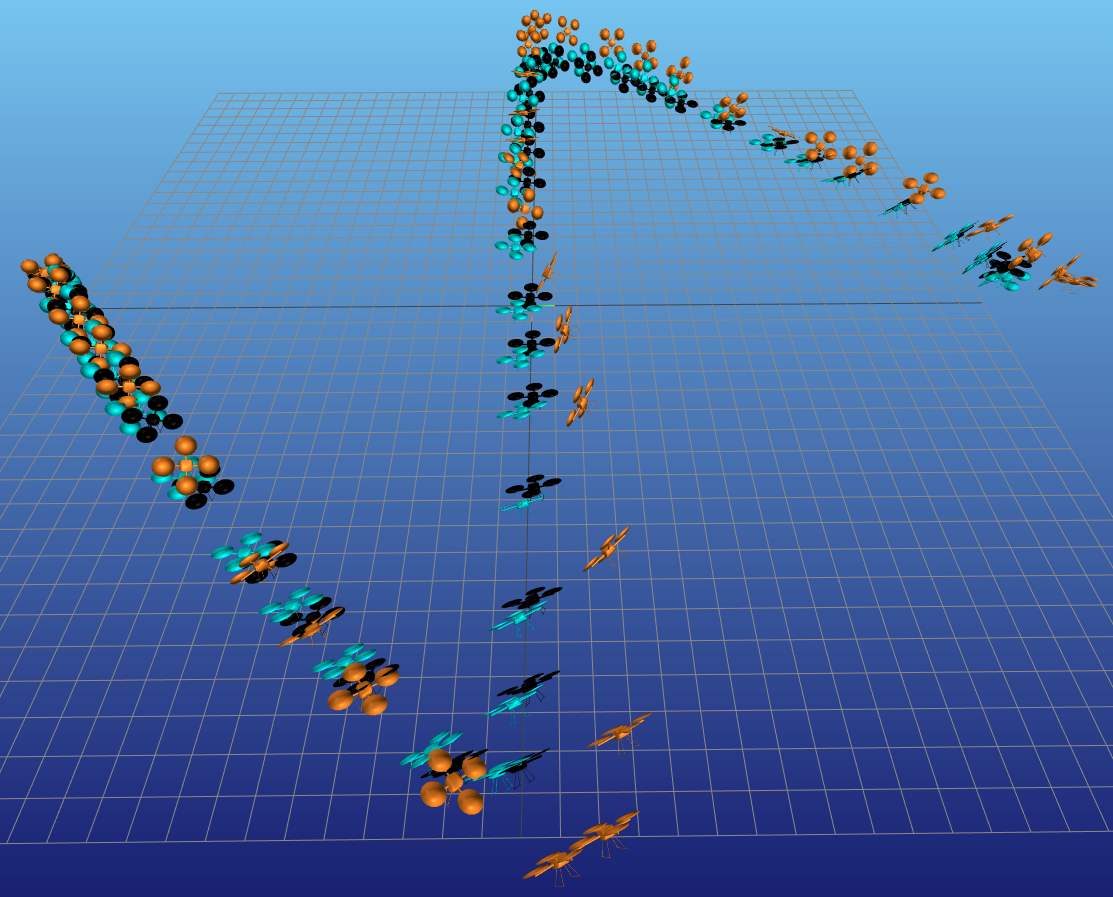
\includegraphics[height=5.2cm]{figures/zig_zag_tracking.png}
%                 \caption{Zig-zag trajectory. The black quadrotors indicate
%                     the reference trajectory generated by iMLQR. The yellow
%                     quadrotors track the reference trajectory using time-varying
%                     MLQR, while the red uses the HFCA controller from
%                     \cite{watterson2020control}.
%                 }
%                 \label{fig:zig-zag}
%             \end{figure}    
%             \begin{figure}[t]
%                 \centering
%                 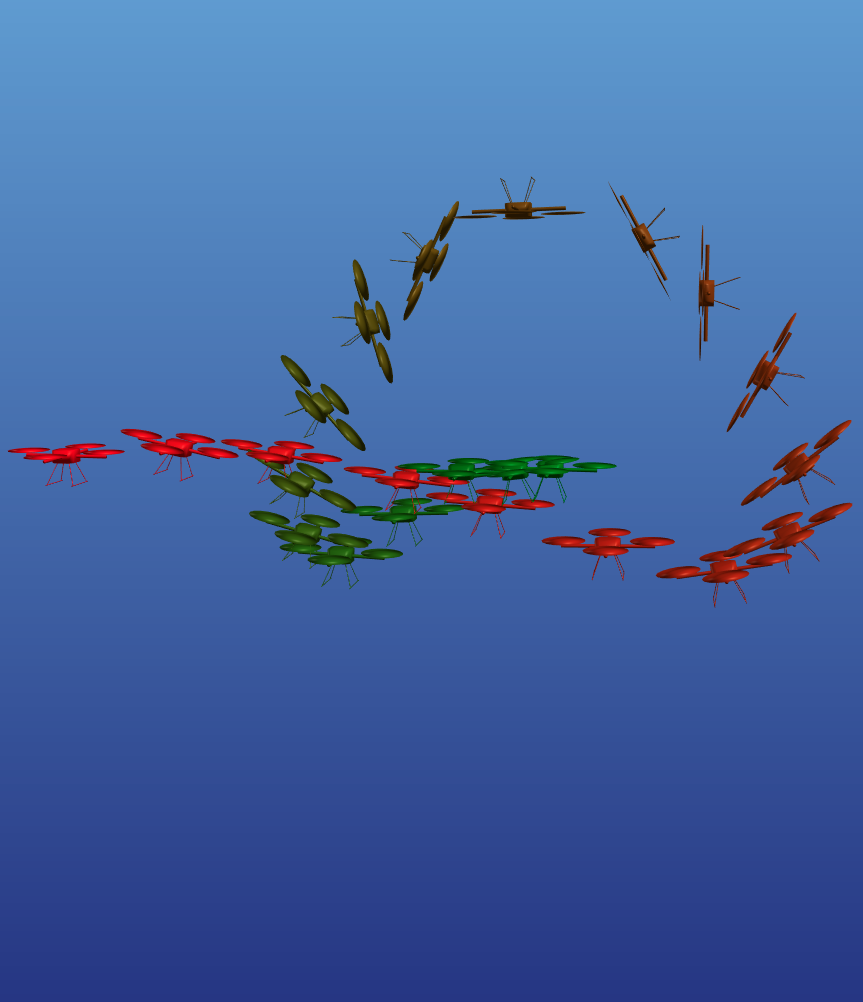
\includegraphics[height=5.2cm,trim={0 3cm 0 0},clip]{figures/quad_flip.png}
%                 \caption{Snapshots of the quadrotor flip trajectory. The
%                     red-colored quadrotors represent the state near t=0 s and the
%                     green-colored quadrotors represent the state near t=5.0 s
%                 }
%                 \label{fig:quad_flip}
%             \end{figure}    
            
%         We set up a fairly simple trajectory optimization problem to achieve a
%         ``zig-zag'' pattern, as shown in Fig. \ref{fig:zig-zag} using cost funtions of
%         the form
%         \begin{multline}
%                   \half \sum_{k \in \mathcal{N}} \ell(x_k, x_\text{nom}, Q_\text{nom}) 
%                 + \half \sum_{k \in \mathcal{W}} \ell(x_k, \bar{x}_k, Q_w) \\
%                 + \half \sum_{k=1} u_k^T R u_k
%         \end{multline}
%         with $\mathcal{W} = \{33,66,101\}$, $\mathcal{N} = \{1:101\} \setminus
%         \mathcal{W}$, and the waypoint positions were $(10,0,1)$,$(-10,0,1)$ and
%         $(0,10,0)$. We compared the two cost functions from Sec.
%         \ref{sec:cost_functions}, using a standard quadratic penalty on the
%         non-quaternion states.
%         \begin{align}
%             \ell_\text{err}(x, \bar{x}, Q) &= \delta x^T Q \delta x \\ 
%             \ell_\text{geo}(x, \bar{x}, Q) &= (x-\bar{x})^T \bar{Q} (x-\bar{x}) + w (1
%                 \pm \bar{q}^T q)
%         \end{align}
%         where $\bar{Q} = \text{diag}(Q_r, \vec{0}_4, Q_v, Q_\omega)$, where
%         $Q_r,Q_v,Q_\omega$ are the weights of $Q$ for position, and linear and angular
%         velocity.
%         We used the following weighting matrices: 
%         $Q_\text{nom} = \text{diag}(10^{-5} I_6,10^{-3} I_6)$, 
%         $Q_w = \text{diag}(10^3 I_3,I_9)$, 
%         $Q_N = \text{diag}(10 I_3, 100 I_3, 10 I_6)$.
%         For the geodesic weights $w$, we used 0, 1, and 10 for the nominal, waypoint, and
%         terminal cost functions, respectively.
        
%         The geodesic cost function performed significantly better than the error
%         quadratic, converging in 10 ms and 13 iterations, compared to 53 ms in 29
%         iterations. In addition to better convergence behavior, the geodesic cost is
%         about half as expensive to compute, which is unsurprising when comparing the
%         gradients and Hessians in Sec. \ref{sec:cost_functions}.

%         \subsubsection{Quadrotor Flip}
% 	    Similar to the previous example, we use a set of waypoints to encourage the
% 	    quadrotor to do a flip. The cost weights for this example were
% 	    \begin{align*}
% 	        Q_\text{nom} &= \text{diag}(10^{-2},10^{-2},5 \!\times\! 10^{-2}, 10^{-3} I_3,
%     	        10^{-3} I_3, 10^{-2} I_3) \\
% 	        Q_w &= \text{diag}(10^3, 10, 10^3, 5000 I_3, I_3, 10 I_3) \\
% 	        Q_N &= \text{diag}(10 I_3, 100 I_3, 10 I_6)  
% 	    \end{align*}
% 	    Four intermediary knotpoints were used to encourage the quadrotor to be at angles
% 	    of \ang{90}, \ang{180}, \ang{270}, and \ang{360}. The quadrotor was constrained
% 	    to stay above the floor and move to a goal state 2 meters away in the $+y$
% 	    direction. The solver is initialized with a dynamically infeasible trajectory
% 	    that linearly interpolates between the initial and final states, rotating the
% 	    quad around the x-axis a full \ang{360}.
	    
% 	    Figure \ref{fig:quad_flip} shows snapshots of the trajectory as generated using
% 	    iMLQR within the ALTRO solver to handle constraints. The trajectory generated by
% 	    iLQR with quaternions and quadratic costs was successful but had a slightly
%         different trajectory. iLQR with Euler angles failed to solve the problem.

%         \subsection{Airplane Barrel Roll}
%         An airplane model with aerodynamic coefficients fit from real wind-tunnel data is
%         tasked to do a barrel roll by setting a high terminal cost for being upside-down,
%         see Fig. \ref{fig:barrellroll}. The solver is initialized with level flight trim
%         conditions. For both the quadrotor flip and the airplane barrel roll, iMLQR
%         converged faster than the pure quaternion version. Despite the extra matrix
%         multiplications and extra Hessian term, it also was faster per iteration than its
%         iLQR counterpart. For these highly aerobatic maneuvers, we achieve, as expected,
%         better performance by correctly leveraging the structure of the rotation group
%         during the optimization routine.

%         \begin{figure}[h]
%             \centering
%             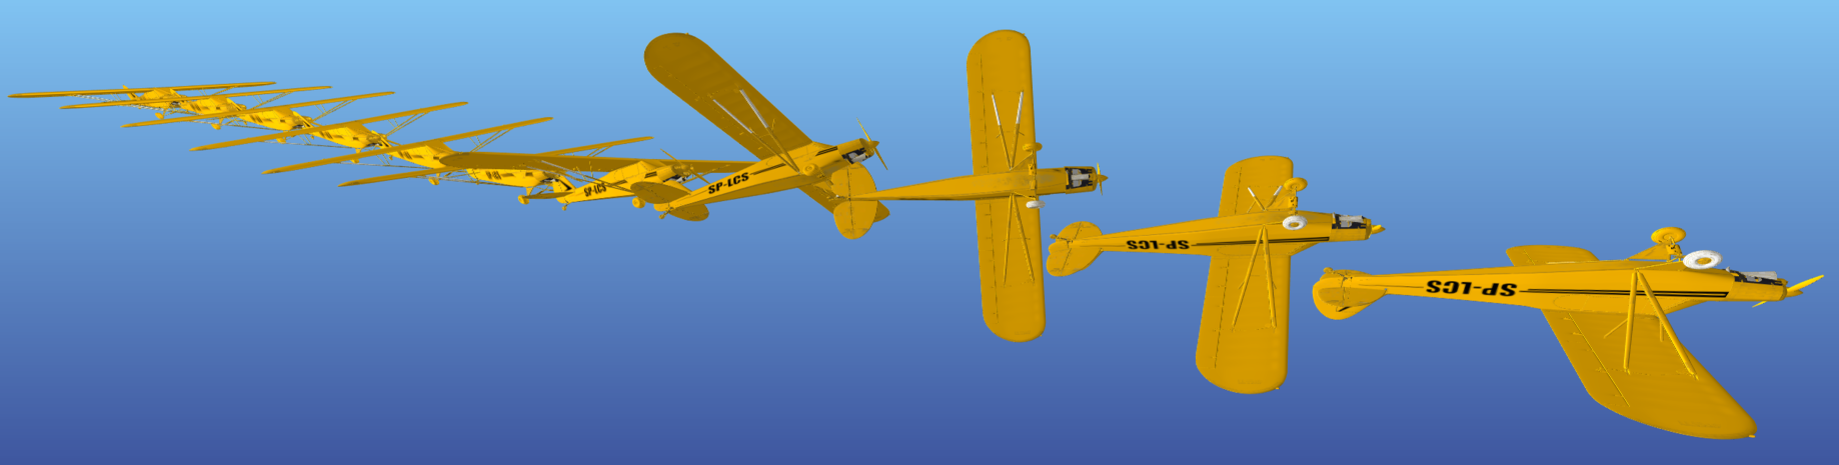
\includegraphics[height=3.5cm]{figures/barrellroll.png}
%             \caption{Barrel roll trajectory computed by iterative MLQR using a terminal cost to encourage an upside-down attitude.}
%             \label{fig:barrellroll}
%         \end{figure}
    
% 	    \begin{figure}[h]
% 	        \centering
% 	        \includegraphics[width=\columnwidth,height=4.5cm]{figures/tracking_err.tikz}
% 	        \caption{Tracking error over time for the zig-zag trajectory using MLQR and the HFCA geometric controller. Band-limited white noise wrenches of variance $w$ are added to the continuous dynamics. }
% 	        \label{fig:tracking_err}
% 	    \end{figure}
%         \vspace{-20pt}

% 	\subsection{Tracking Control}
% 	    This section provides examples using MLQR for tracking and stabilizing control
% 	    for a quadrotor. We compare our MLQR controller to HFCA, a state-of-the-art
% 	    geometric tracking controller \cite{watterson2020control} based on the Hopf
% 	    Fibration.
	    
% 	    \subsubsection{MLQR Stabilization}
% 	    To test robustness and the domain of attraction of the MLQR controller, a
% 	    quadrotor is linearized about hover at the origin and initialized from states
% 	    uniformly sampled in $[-1,1]$ for position, $[-5,5]$ for linear and angular
% 	    velocities, and uniformly over the entire space of rotations. The success rates
% 	    for 2000 trials are given in Table \ref{tab:mlqr_success}, where success is
% 	    defined as the terminal error (calculated using \eqref{eq:state_error}) being
% 	    within a unit ball of radius 0.1 after 10.0 seconds. To further analyze the
% 	    basins of attraction, we uniformly sampled over only roll (which goes singular at
% 	    \ang{90} for our Euler angle representation), and yaw. The results are shown in
% 	    Fig. \ref{fig:mlqr_basin}, where the plotted contours are the convex hull of the
% 	    successfully stabilized initial conditions.
	    
% 	    MLQR slightly exceeds the robustness of the HFCA geometric controller, while also
% 	    being more generally applicable, easier to tune, and easier to implement. It is
% 	    also noteworthy that na\"ively using LQR with quaternions (incorrectly treating
% 	    them as vectors) results in poorer performance than Euler angles, clearly
% 	    demonstrating the value of the methodology presented in the current paper.
	    
% 	    \subsubsection{MLQR Tracking}
% 	    Time-varying MLQR is used to track the zig-zag trajectory generated in the
% 	    previous section. %The controller calculated the gains at $0.01 s$ intervals, and
% 	    used zero-order-hold between intervals. To test tracking performance, zero-mean
% 	    Gaussian noise was added as force and moments applied to the quadrotor.
	    
% 	    The trajectories and tracking error for MLQR and HFCA are shown in Figs.
% 	    \ref{fig:zig-zag}, and \ref{fig:tracking_err}. While the MLQR controller
% 	    dramatically out-performs HFCA, we found no significant difference in performance
% 	    between MLQR and LQR using either roll-pitch-yaw Euler angles or a quaternion.
% 	    Since the tracking controller only deals with relatively small state and attitude
% 	    errors, this is unsurprising. Additionally, we found the MLQR controller ran
%         about 20x faster than the HFCA controller.

% 	    \begin{figure*}[ht]
% 	        \begin{minipage}{0.60\linewidth}
%                 \centering
%                 \includegraphics[height=6.6cm,width=\textwidth]{figures/mlqr_basin.tikz}
%                 \caption{Basins of attraction of 4 stabilizing controllers for yaw and roll, calculated from 2000 sample points (shown in black). All points within each contour were successfully stabilized by the controller.}
%                 \label{fig:mlqr_basin}
%             \end{minipage}
% 	        \hspace{0.05\linewidth}
%             \begin{minipage}{0.34\linewidth}
%                 \centering
%                 \begin{tabular}{cc}
%                     \toprule
%                     \textbf{Method} & \textbf{Success} \\
%                     \midrule
%                     Quat & 61\% \\
%                     RPY  & 80\% \\
%                     HFCA & 97\% \\
%                     MLQR & 99\% \\
%                     \bottomrule
%                 \end{tabular}
%                 \caption{Success rate for Monte-Carlo analysis of quadrotor stabilization for 2000 initial conditions uniformly over position, orientation, and linear and angular velocities.}
%                 \label{tab:mlqr_success}
%             \end{minipage}
%         \end{figure*}

% \section{Conclusions} \label{sec:conclusion}
%     We have presented a general, unified method for planning and control on rigid-body
%     systems with arbitrary attitude using standard linear algebra and vector calculus. By
%     applying these methods to LQR to correctly account for the group structure of
%     rotations, we have matched or exceeded the performance of a state-of-the-art
%     geometric controller designed specifically for quadrotors, while being more general,
%     requiring less system-dependent tuning, having less computational overhead, and being
%     easier to implement.
    
%     We have also demonstrated a straight-forward way to adapt nonlinear trajectory
%     optimization techniques to work with quaternion-valued states. For these problems, we
%     found the geodesic distance between quaternions \eqref{eq:quat_geodesic} to be
%     computationally efficient and provide excellent convergence in practice. We recommend
%     the use of unit quaternions within planning and control algorithms for their
%     simplicity, computational efficiency, and lack of singularities. We further recommend
%     the use of Rodrigues parameters, or the Cayley map, as the quaternion error state.
    
%     Future areas of research include the application of these methodologies to more
%     complex multi-body floating-base robots, such as humanoids and quadrupeds, as well as
%     more in-depth analysis of the convergence behavior of the algorithms proposed in the
%     current work.
    
% \paragraph{Acknowledgements}
% This material is based upon work supported by the National Science Foundation Graduate
% Research Fellowship Program under Grant No. DGE-1656518. Any opinions, findings, and
% conclusions or recommendations expressed in this material are those of the author(s) and
% do not necessarily reflect the views of the National Science Foundation


\printbibliography

\end{document}